\section{Risk-Certified Query Optimization}
\label{sec:optimizer}

\begin{figure}[t]
\centering
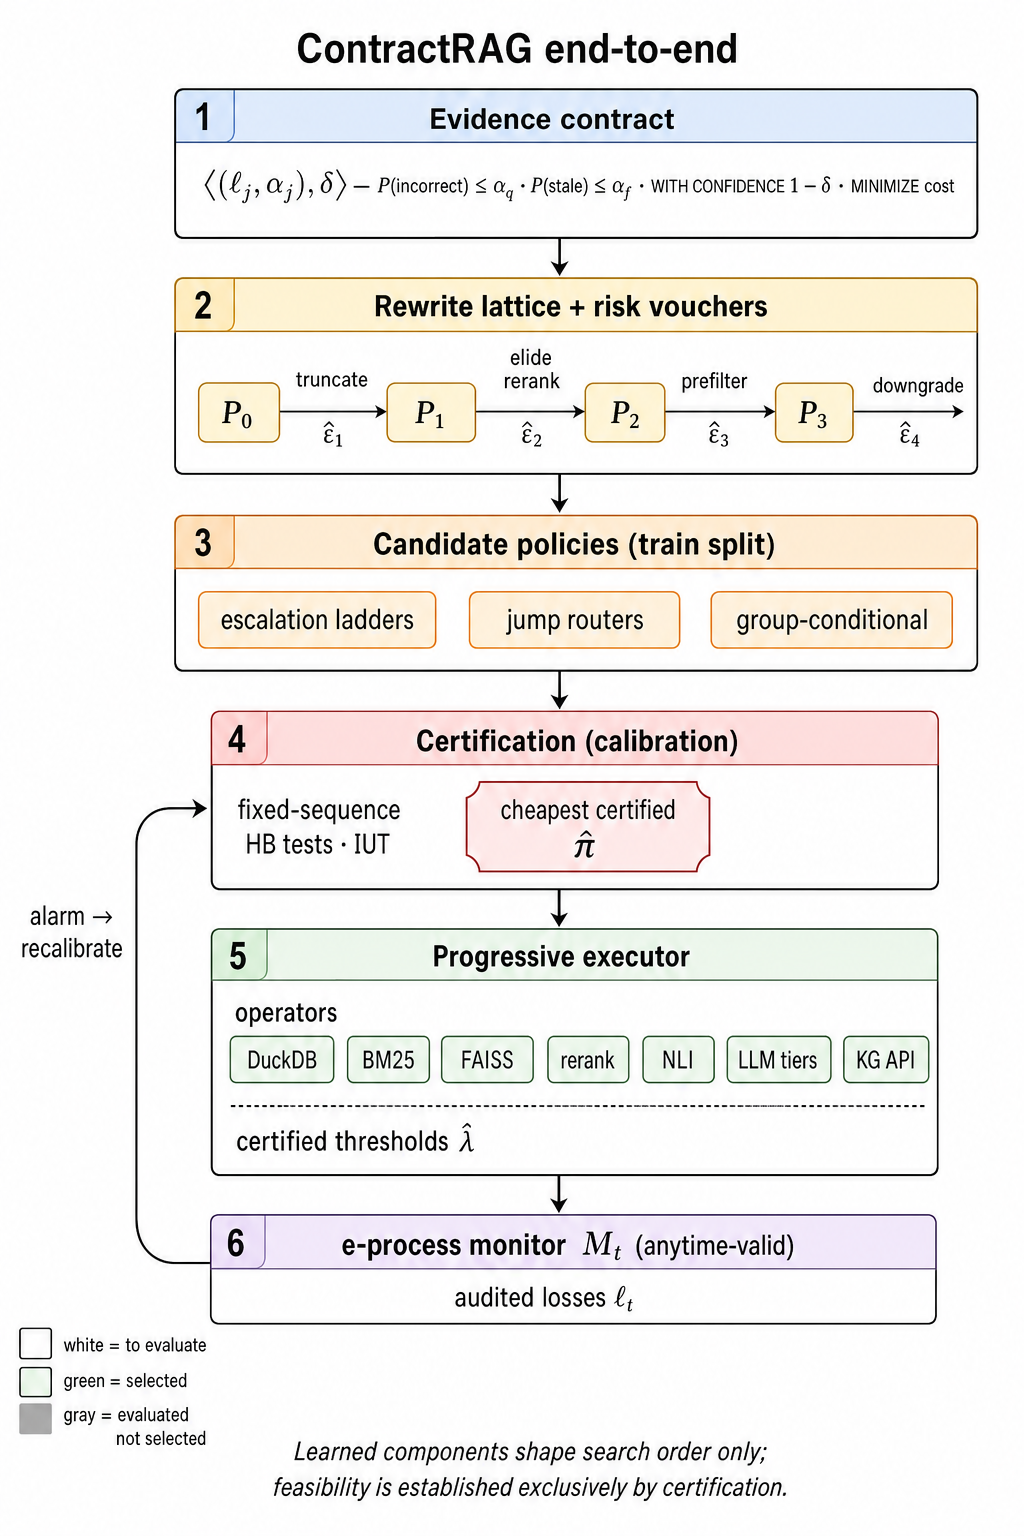
\includegraphics[width=\columnwidth]{figures/fig_arch_imagegen.png}
\caption{\system\ end to end. The application declares a contract (blue);
the rewrite layer generates a voucher-annotated plan lattice and the
policy layer lifts it into adaptive candidates on the train split
(orange); the certification layer walks the candidates with
fixed-sequence tests on the calibration split and deploys the cheapest
certified policy (red); the executor runs it progressively over the
physical operators (green) while the e-process monitor audits realized
losses and triggers recalibration on drift (violet). Learned components
shape only the search order; feasibility is established exclusively by
the red layer.}
\Description{The ContractRAG architecture: evidence contract, rewrite
and policy generation, fixed-sequence certification, progressive
execution, monitoring, and recalibration.}
\label{fig:arch}
\end{figure}


\system separates plan search from authorization to deploy
(Fig.~\ref{fig:arch}). The rewrite and policy layers use a training split
to generate and order candidates. A certification layer touches an
independent calibration split once and returns the cheapest policy in the
certified prefix. Search estimates may therefore be inaccurate without
invalidating the contract.

\subsection{Non-equivalent rewrites and risk vouchers}
\label{sec:rewrites}

\begin{figure*}[t]
\centering
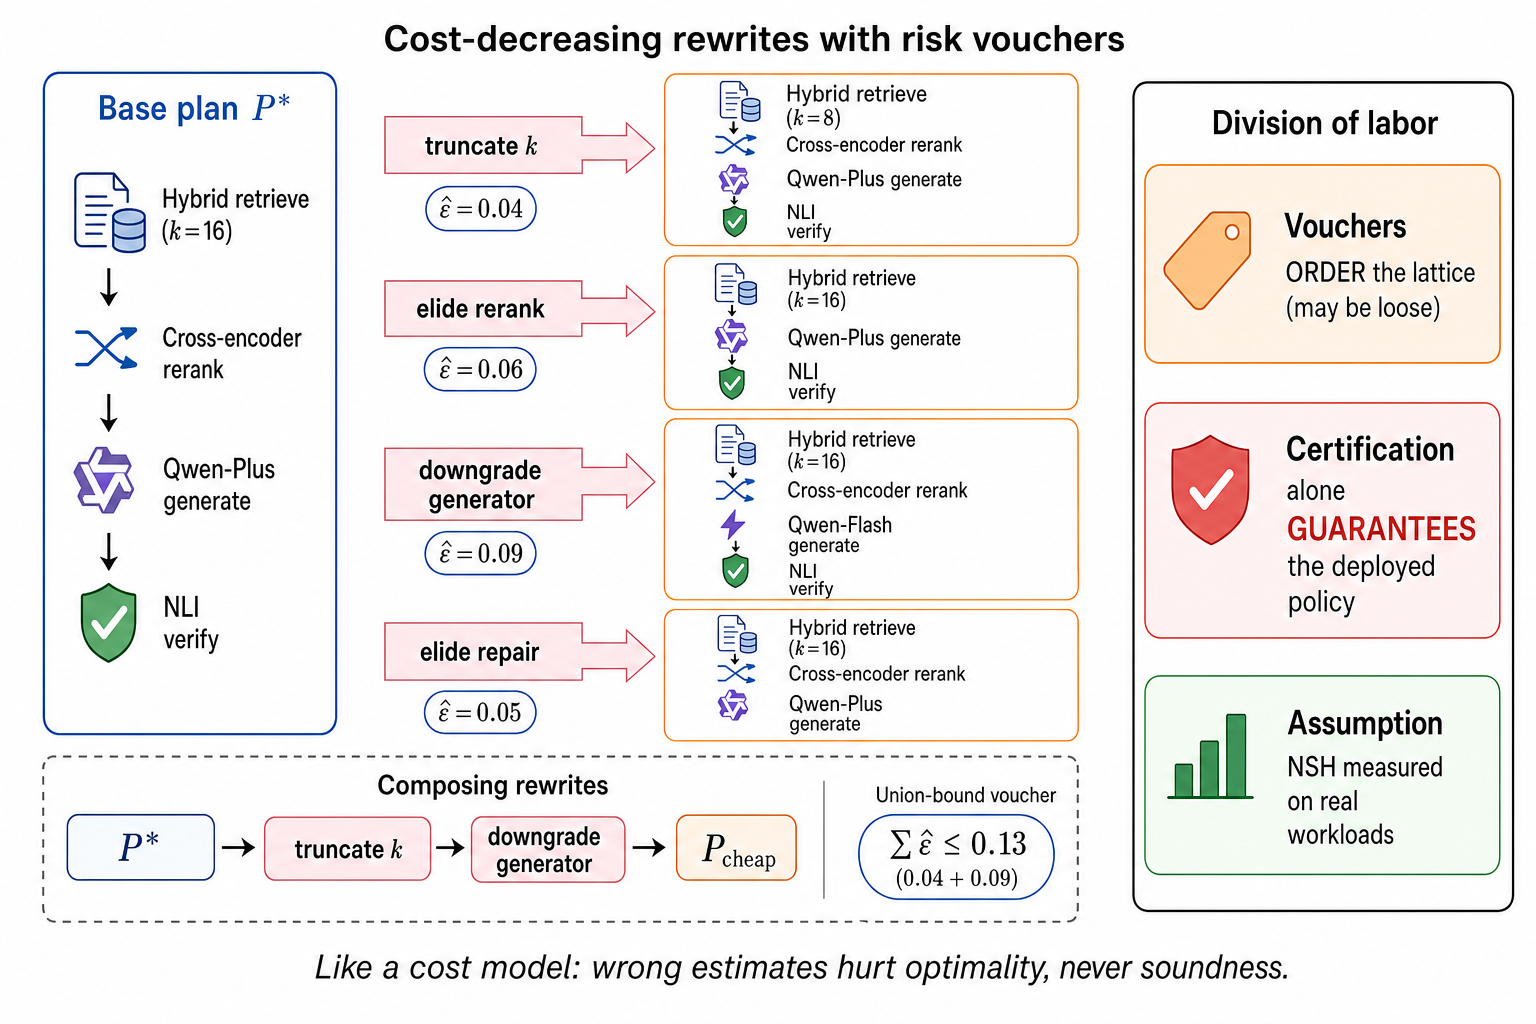
\includegraphics[width=0.95\textwidth]{figures/fig_rewrites_imagegen.png}
\caption{Cost-decreasing rewrites with risk vouchers. From a base plan
$P^\ast$ (left), each rewrite produces a cheaper variant annotated with a
Clopper--Pearson harm bound $\hat\eps$ (center). Vouchers compose
assumption-free along rewrite chains via the telescoping bound of
Proposition~\ref{prop:composition}. The division of
labor (right) mirrors classical optimizers: vouchers order the search
space like a cost model; only direct certification of the deployed
policy establishes the contract (Definition~\ref{def:voucher},
Proposition~\ref{prop:composition}).}
\Description{A base retrieval-augmented plan is transformed by
cost-reducing rewrites. Risk vouchers annotate rewrite edges and guide
the search, while direct certification authorizes the deployed policy.}
\label{fig:rewrites}
\end{figure*}


The optimizer applies cost-reducing rewrites: retrieval truncation,
reranker elision, structured pre-filter pushdown, generator downgrade, and
repair elision. Since these rewrites are not equivalence preserving,
\system attaches a risk estimate to each edge of the plan lattice.

\begin{definition}[Risk voucher]
\label{def:voucher}
For loss $\ell$ and a rewrite $R:P\mapsto P'$, define its harm probability
as $\rho(R;P)=\Prob_q(\ell(P',q)>\ell(P,q))$. An
$(\hat\eps,\delta_r)$ voucher is a Clopper--Pearson upper confidence bound
$\hat\eps$ for $\rho$, estimated from paired training executions of $P$
and $P'$.
\end{definition}

Voucher composition must account for rewrite interactions. Consider
$P_0\xrightarrow{R_1}P_1\cdots\xrightarrow{R_m}P_m$, with every edge
measured against its actual predecessor.

\begin{proposition}[Path voucher]
\label{prop:composition}
If edge $i$ has voucher $(\hat\eps_i,\delta_r)$, then with probability at
least $1-m\delta_r$,
\[
\Prob(\ell(P_m,q)>\ell(P_0,q))\leq\sum_{i=1}^{m}\hat\eps_i .
\]
\end{proposition}
\begin{proof}
Whenever $\ell(P_m,q)-\ell(P_0,q)>0$, at least one term in the telescoping
sum $\sum_i[\ell(P_i,q)-\ell(P_{i-1},q)]$ is positive. A union bound first
over these harm events and then over the confidence bounds proves the
claim.
\end{proof}

The path construction requires no assumption about synergistic harm.
\system also conditions pushdown vouchers on estimated pool selectivity:
queries are divided into selectivity strata and a confidence bound is
estimated per stratum, with Bonferroni correction across strata. Vouchers
only rank candidates; the selected policy is tested directly in
\S\ref{sec:certification}.

\subsection{Access paths and shared subplans}
\label{sec:planner}

A hybrid QA query often joins structured rows $S$ with linked text $T$.
\emph{Table-first} selects rows and searches only their passage pool;
\emph{text-first} searches the full pool and joins passages back to rows.
The first is cheaper when the predicate sharply reduces the pool, while
the second preserves recall for vague predicates. Before retrieval,
\system obtains row and passage counts from the link table and computes
$\sigma=|T_{\mathrm{push}}|/|T_{\mathrm{full}}|$. A measured linear cost
model and a training-split recall model choose the cheapest path whose
predicted recall meets the target. This choice parameterizes the plan
lattice, but direct certification remains the feasibility check.

Retrieval results are independent of the generator. \system materializes
each query--rung retrieval result once and shares it across generators and
policy candidates. Certification then evaluates policies over a common
execution matrix instead of issuing additional model calls.

\subsection{Adaptive policy families}
\label{sec:families}

The rewrite lattice yields a cost-ascending ladder
$P_0\prec\cdots\prec P_{L-1}$. Rung $j$ emits a sufficiency score
$s_j(q)\in[0,1]$ from runtime features such as retrieval margins, reranker
scores, citation coverage, evidence age, and entailment. Per-rung logistic
models are trained only on the training split. \system constructs:
\begin{itemize}
  \item \textbf{fixed policies}, one for each rung;
  \item \textbf{progressive policies}, which execute upward and stop at the
  first rung with $s_j(q)\geq\lambda_j$; and
  \item \textbf{routing policies}, which jump to
  $\arg\max_j(s_j(q)-\lambda\bar c_j)$.
\end{itemize}
Threshold and utility grids produce a finite candidate set $\Pi$. Policies
may also be specialized by a query group known at execution time.

\subsection{Selection-valid certification}
\label{sec:certification}

For candidate $\pi$ and constraint $j$, let $\hat R_j(\pi)$ be its loss on
$n$ calibration queries. We test
$H_0^{(j)}(\pi):R_j(\pi)>\alpha_j$ using the Hoeffding--Bentkus
p-value~\cite{bentkus2004hoeffding,angelopoulos2021ltt}
\[
p_\pi^{(j)}=\min\!\left\{
e^{-n h_1(\hat R_j\wedge\alpha_j,\alpha_j)},\
e\,\Prob[\mathrm{Bin}(n,\alpha_j)\leq\lceil n\hat R_j\rceil]
\right\},
\]
where $h_1$ is Bernoulli KL divergence. For multiple constraints, the
infeasibility null is the union $\bigcup_jH_0^{(j)}$. The
intersection--union test rejects it only when every $p_\pi^{(j)}\leq
\delta$, so no Bonferroni split across constraints is required.

Candidates are ordered by training-split risk, with training cost breaking
ties. This order is fixed before calibration. The optimizer tests candidates
in order, stops at the first non-rejection, and returns the lowest-cost
candidate among those certified before the stop.

\begin{theorem}[Contract validity]
\label{thm:validity}
For any candidate count, score quality, and query distribution, the
returned policy $\hat\pi$ satisfies
\[
\Prob\!\left(R_j(\hat\pi)\leq\alpha_j\ \text{for every }j\right)
\geq1-\delta .
\]
\end{theorem}
\begin{proof}
Let $\pi_{k^\star}$ be the first infeasible candidate in the fixed order.
The procedure can return an infeasible policy only if it reaches and
falsely certifies $\pi_{k^\star}$. Its intersection--union test has size at
most $\delta$. Later candidates are unreachable without this event, and
choosing among the certified prefix introduces no further error.
\end{proof}

The ordering determines power, not validity. A better risk model reaches
cheaper feasible candidates before the first failure; a poor model may
stop early but cannot authorize an infeasible policy with probability
greater than $\delta$. The certification pass is vectorized over the
materialized execution matrix and requires no extra LLM calls.
